\documentclass{article}

\relax% header
	\usepackage{aistats2022_author_response}
		\usepackage[utf8]{inputenc} % allow utf-8 input
		\usepackage[T1]{fontenc}    % use 8-bit T1 fonts
		\usepackage{hyperref}       % hyperlinks
		\usepackage{url}            % simple URL typesetting
		\usepackage{booktabs}       % professional-quality tables
		\usepackage{amsfonts}       % blackboard math symbols
		% \usepackage{nicefrac}       % compact symbols for 1/2, etc.
		\usepackage{microtype}      % microtypography
		% \usepackage{xcolor}         % define colors in text
		\usepackage{xspace}         % fix spacing around commands

	\relax % tikz
		\usepackage[dvipsnames]{xcolor}
		\usepackage{tikz}
			\usetikzlibrary{positioning,fit,calc, decorations, arrows, shapes, shapes.geometric}
			\usetikzlibrary{cd}

			%%%%%%%%%%%%
			\tikzset{AmpRep/.style={ampersand replacement=\&}}
			\tikzset{center base/.style={baseline={([yshift=-.8ex]current bounding box.center)}}}
			\tikzset{paperfig/.style={center base,scale=0.9, every node/.style={transform shape}}}

			% Node Stylings
			\tikzset{dpadded/.style={rounded corners=2, inner sep=0.7em, draw, outer sep=0.3em, fill={black!50}, fill opacity=0.08, text opacity=1}}
			\tikzset{dpad0/.style={outer sep=0.05em, inner sep=0.3em, draw=gray!75, rounded corners=4, fill=black!08, fill opacity=1, align=center}}
			\tikzset{dpadinline/.style={outer sep=0.05em, inner sep=2.5pt, rounded corners=2.5pt, draw=gray!75, fill=black!08, fill opacity=1, align=center, font=\small}}

		 	\tikzset{dpad/.style args={#1}{every matrix/.append style={nodes={dpadded, #1}}}}
			\tikzset{light pad/.style={outer sep=0.2em, inner sep=0.5em, draw=gray!50}}

			\tikzset{arr/.style={draw, ->, thick, shorten <=3pt, shorten >=3pt}}
			\tikzset{arr0/.style={draw, ->, thick, shorten <=0pt, shorten >=0pt}}
			\tikzset{arr1/.style={draw, ->, thick, shorten <=1pt, shorten >=1pt}}
			\tikzset{arr2/.style={draw, ->, thick, shorten <=2pt, shorten >=2pt}}

			\newcommand\cmergearr[5][]{
				\draw[arr, #1, -] (#2) -- (#5) -- (#3);
				\draw[arr, #1, shorten <=0] (#5) -- (#4);
				}
			\newcommand\mergearr[4][]{
				\coordinate (center-#2#3#4) at (barycentric cs:#2=1,#3=1,#4=1.2);
				\cmergearr[#1]{#2}{#3}{#4}{center-#2#3#4}
				}
			\newcommand\cunmergearr[5][]{
				\draw[arr, #1, -, shorten >=0] (#2) -- (#5);
				\draw[arr, #1, shorten <=0] (#5) -- (#3);
				\draw[arr, #1, shorten <=0] (#5) -- (#4);
				}
			\newcommand\unmergearr[4][]{
				% \coordinate (center-#2#3#4) at (barycentric cs:#2=1.2,#3=1,#4=1);
				\coordinate (center-#2#3#4) at (barycentric cs:#2=2,#3=1,#4=1);
				\cunmergearr[#1]{#2}{#3}{#4}{center-#2#3#4}
				}
			\newcommand\lab[1]{(#1)(lab-#1)}
			\tikzset{alternative/.style args={#1|#2|#3}{name=#1, circle, fill, inner sep=1pt,label={[name={lab-#1},gray!30!black, inner sep=1pt]#3:\scriptsize #2}} }
			\tikzset{tpt/.style args={#1|#2}{alternative={#1|#2|below}} }
			\tikzset{Dom/.style args={#1[#2] (#3) around #4}{dpadded, name=#3, label={[name={lab-#3},align=center,label distance=-1.9em, shading = axis, top color=white, bottom color=black!04, #2]120:#1}, fit={ #4 }, inner sep=0.5em}}

	\relax % Most oli packages
	    \usepackage{mathtools}
	    \usepackage{amssymb}
			\DeclareMathSymbol{\shortminus}{\mathbin}{AMSa}{"39}
	    \usepackage{bbm}
	    \usepackage{graphicx}
	    \usepackage{scalerel}
	    \usepackage{enumitem}
	    \usepackage{nicefrac}\let\nf\nicefrac

	    \usepackage{color}
	    %\usepackage{stmaryrd}
	    \usepackage{hyperref} % Load before theorems...
	        \hypersetup{colorlinks=true, linkcolor=blue!75!black, urlcolor=magenta, citecolor=green!50!black}

	\usepackage{amsthm,thmtools} % Theorem Packages
		\usepackage[noabbrev,nameinlink,capitalize]{cleveref}
	    \theoremstyle{plain}
	    \newtheorem{theorem}{Theorem}
		\newtheorem{coro}{Corollary}[theorem]
	    \newtheorem{prop}[theorem]{Proposition}
	    \newtheorem{claim}{Claim}
	    \newtheorem{remark}{Remark}
	    \newtheorem{lemma}[theorem]{Lemma}
	    \theoremstyle{definition}
	    % \newtheorem{defn}{Definition}
	    % \declaretheorem[name=Definition]{defn}
	    \declaretheorem[name=Definition, qed=$\square$]{defn}

		\crefname{defn}{Definition}{Definitions}
		\crefname{prop}{Proposition}{Propositions}

	\relax %%%%%%%%% GENERAL MACROS %%%%%%%%
	    \let\Horig\H
		\let\H\relax
		\DeclareMathOperator{\H}{\mathrm{H}} % Entropy
		\DeclareMathOperator{\I}{\mathrm{I}} % Information
		\DeclareMathOperator*{\Ex}{\mathbb{E}} % Expectation
		\DeclareMathOperator*{\EX}{\scalebox{1.5}{$\mathbb{E}$}}

	    \newcommand{\mat}[1]{\mathbf{#1}}
	    \DeclarePairedDelimiterX{\infdivx}[2]{(}{)}{%
			#1\;\delimsize\|\;#2%
		}
		\newcommand{\thickD}{I\mkern-8muD}
		\newcommand{\kldiv}{\thickD\infdivx}
		\newcommand{\tto}{\rightarrow\mathrel{\mspace{-15mu}}\rightarrow}

		\newcommand{\datadist}[1]{\Pr\nolimits_{#1}}
		% \newcommand{\datadist}[1]{p_\text{data}}

		\makeatletter
		\newcommand{\subalign}[1]{%
		  \vcenter{%
		    \Let@ \restore@math@cr \default@tag
		    \baselineskip\fontdimen10 \scriptfont\tw@
		    \advance\baselineskip\fontdimen12 \scriptfont\tw@
		    \lineskip\thr@@\fontdimen8 \scriptfont\thr@@
		    \lineskiplimit\lineskip
		    \ialign{\hfil$\m@th\scriptstyle##$&$\m@th\scriptstyle{}##$\hfil\crcr
		      #1\crcr
		    }%
		  }%
		}
		\makeatother
		\newcommand\numberthis{\addtocounter{equation}{1}\tag{\theequation}}

	\relax %%%%%%%%%   PDG  MACROS   %%%%%%%%
		\newcommand{\ssub}[1]{_{\!_{#1}\!}}
		% \newcommand{\bp}[1][L]{\mat{p}_{\!_{#1}\!}}
		% \newcommand{\bP}[1][L]{\mat{P}_{\!_{#1}\!}}
		\newcommand{\bp}[1][L]{\mat{p}\ssub{#1}}
		\newcommand{\bP}[1][L]{\mat{P}\ssub{#1}}
		\newcommand{\V}{\mathcal V}
		\newcommand{\N}{\mathcal N}
		\newcommand{\Ed}{\mathcal E}

        \newcommand{\balpha}{\boldsymbol\alpha}
        \newcommand{\bbeta}{\boldsymbol\beta}

		\DeclareMathAlphabet{\mathdcal}{U}{dutchcal}{m}{n}
		\DeclareMathAlphabet{\mathbdcal}{U}{dutchcal}{b}{n}
		\newcommand{\dg}[1]{\mathbdcal{#1}}
		\newcommand{\PDGof}[1]{{\dg M}_{#1}}
		\newcommand{\UPDGof}[1]{{\dg N}_{#1}}
		\newcommand\VFE{\mathit{V\mkern-4mu F\mkern-4.5mu E}}

		\newcommand\Inc{\mathit{Inc}}
		\newcommand{\IDef}[1]{\mathit{IDef}_{\!#1}}
		% \newcommand{\ed}[3]{%
		% 	\mathchoice%
		% 	{#2\overset{\smash{\mskip-5mu\raisebox{-3pt}{${#1}$}}}{\xrightarrow{\hphantom{\scriptstyle {#1}}}} #3} %display style
		% 	{#2\overset{\smash{\mskip-5mu\raisebox{-3pt}{$\scriptstyle {#1}$}}}{\xrightarrow{\hphantom{\scriptstyle {#1}}}} #3}% text style
		% 	{#2\overset{\smash{\mskip-5mu\raisebox{-3pt}{$\scriptscriptstyle {#1}$}}}{\xrightarrow{\hphantom{\scriptscriptstyle {#1}}}} #3} %script style
		% 	{#2\overset{\smash{\mskip-5mu\raisebox{-3pt}{$\scriptscriptstyle {#1}$}}}{\xrightarrow{\hphantom{\scriptscriptstyle {#1}}}} #3}} %scriptscriptstyle
		\newcommand{\ed}[3]{#2%
		  \overset{\smash{\mskip-5mu\raisebox{-1pt}{$\scriptscriptstyle
		        #1$}}}{\rightarrow} #3}

	    \newcommand{\nhphantom}[2]{\sbox0{\kern-2%
			\nulldelimiterspace$\left.\delimsize#1\vphantom{#2}\right.$}\hspace{-.97\wd0}}
			% \nulldelimiterspace$\left.\delimsize#1%
			% \vrule depth\dp#2 height \ht#2 width0pt\right.$}\hspace{-.97\wd0}}
		\makeatletter
		\newsavebox{\abcmycontentbox}
		\newcommand\DeclareDoubleDelim[5]{
		    \DeclarePairedDelimiterXPP{#1}[1]%
				{% box must be saved in this pre code
					\sbox{\abcmycontentbox}{\ensuremath{##1}}%
				}{#2}{#5}{}%
			    %%% Correct spacing, but doesn't work with externalize.
				% {\nhphantom{#3}{##1}\hspace{1.2pt}\delimsize#3\mathopen{}##1\mathclose{}\delimsize#4\hspace{1.2pt}\nhphantom{#4}{##1}}
				%%% Fast, but wrong spacing.
				% {\nhphantom{#3}{~}\hspace{1.2pt}\delimsize#3\mathopen{}##1\mathclose{}\delimsize#4\hspace{1.2pt}\nhphantom{#4}{~}}
				%%% with savebox.
			    {%
					\nhphantom{#3}{\usebox\abcmycontentbox}%
					\hspace{1.2pt} \delimsize#3%
					\mathopen{}\usebox{\abcmycontentbox}\mathclose{}%
					\delimsize#4\hspace{1.2pt}%
					\nhphantom{#4}{\usebox\abcmycontentbox}%
				}%
		}
		\makeatother
		\DeclareDoubleDelim
			\SD\{\{\}\}
		\DeclareDoubleDelim
			\bbr[[]]
		% \DeclareDoubleDelim
		% 	\aar\langle\langle\rangle\rangle
		\makeatletter
		\newsavebox{\aar@content}
		\newcommand\aar{\@ifstar\aar@one@star\aar@plain}
		\newcommand\aar@one@star{\@ifstar\aar@resize{\aar@plain*}}
		\newcommand\aar@resize[1]{\sbox{\aar@content}{#1}\scaleleftright[3.8ex]
			{\Biggl\langle\!\!\!\!\Biggl\langle}{\usebox{\aar@content}}
			{\Biggr\rangle\!\!\!\!\Biggr\rangle}}
		\DeclareDoubleDelim
			\aar@plain\langle\langle\rangle\rangle
		\makeatother


% take off one-page restriction, for draft
% \makeatletter
% 	\gdef\@outputpage{%
% 	  \stepcounter{pagecount}%
% 	  \ifnum\value{pagecount}>1\relax%
% 	    % Do not output the page
% 	    \PackageWarning{aistats_author_response}{Only one page allowed! Discarding any extra output.}
% 	  \else \fi
% 	  \latex@outputpage%
% 	}
% 	\makeatother

\definecolor{revcolor}{rgb}{0.5, 0.5, 0.0}
\newcommand\revc[1]{{\color{revcolor}#1}}

\begin{document}


\textbf{Confidences.}
\revc{Reviewers \#5} and \revc{\#7} raise an important weakness of the presentation: we ought to say more about the confidence parameters, particularly $\beta$.
% $\beta$ (and clarify the auxiliary role of $\alpha$).
% Choosing $\beta=0$ for a cpd $p$ means that $p$ is effectively ignored, in the sense that a PDG is semantically equivalent to one without $p$.
%TODO:
% doesn't matter WHICH cpd (could replace)
% this PDG becomes equivalent to the same PDG without the edge labeled $p$.
Chosing $\beta=0$ in a cpd $p$
means that $p$ is effectively ignored, in the sense that such a PDG is semantically equivalent to one in which the edge is attached to a different cpd $q \ne p$.
On the other hand, setting $\beta$ to a large real number (or $\infty$) indicates high (or absolute) confidence in $p$.  This is particularly appropriate if $p$ is a trusted empirical distribution
and the other edges are randomly initialized networks.
In other cases (see below), a different choice of $\beta$ may be appropriate.
Figure 1 doubles as a map of how $\beta$
affects the loss for generative models.



% Reviewer \#7 asks about our choice of default values of $\beta\!=\! 1$ and $\alpha\!=\! 0$.
\revc{Reviewer \#7} asks about our choice of default values of $\beta$ and $\alpha$.
The default $\beta\!=\! 1$ is just a convenient choice of units---what’s important are the magnitudes of $\beta$ relative to each other (and to $\gamma$, for $\gamma$-inconsistency).
% (and to $\gamma>0$, for $\gamma$-inconsistency).
% \textbf{Alphas.}
%%% v0
% The default choice of $\alpha$ is even \emph{less} consequential, because $\alpha$ does not affect the inconsistency $\aar{\dg M}$ (it only affects the $\gamma$-inconsistency $\aar{\dg M}_\gamma$ for $\gamma > 0$, which we use only where $\alpha$ more carefully in sections 7 and 8).
%%% v1
% The default choice of $\alpha$ is even \emph{less} consequential, because $\alpha$ does not affect the inconsistency $\aar{\dg M}$, but only the $\gamma$-inconsistency $\aar{\dg M}_\gamma$ for $\gamma > 0$, which is used only in sections 7 and 8 and with more precise selection of $\alpha$.
%%% v2
% The default choice of $\alpha$ is even \emph{less} consequential, because $\alpha$ does not affect the inconsistency $\aar{\dg M}$---only the $\gamma$-inconsistency $\aar{\dg M}_\gamma$ for $\gamma > 0$.
%%% v3: deleted altogether, moved to next sentence
%
% Although we find zero to be the most natural default, it is
% We chose a default of $\alpha=0$ becuase we view it as the the most neutral choice%
% We chose a default of $\alpha\!=\! 0$ becuase it is relatively neutral%
% We chose a default of $\alpha\!=\! 0$ to suggest minimal impact%
We chose a default of $\alpha\!=\! 0$ to suggest a lack of causal modeling%
% \ but in retrospect,
% (the qualitative score reduces to negative entropy)%
, but in retrospect it was a mistake to have a default at all; %---%
% as Reviewer \#7 points out, $\alpha\!=\! 0$ default is inappropriate in cases where the modeler ought to be more confident of the functional dependencies.
as \revc{Reviewer \#7} points out, $\alpha\!=\! 0$ is inappropriate when the modeler has reason to be confident in a functional dependence.
%
% This issue is easly fixed though, since all results hold for every choice of alpha except in the two places where we explicitly choose a different value of $\alpha$.
% This is a problem, but only a superficial one: our results hold for every choice of alpha except
This is only a superficial problem.
% Because $\aar{\dg M}$ does not depend on $\balpha$,
Since $\aar{\dg M}$ does not depend on $\balpha$,
% Our results hold for all choices of $\balpha$, except for in Prop 13 where we explicitly set $\balpha \!=\! \bbeta$ to get the correspondence with factor graphs, and at the end of \S8 where we set $\alpha \!=\! 1$ to enforce independence.
our results hold for all choices of $\balpha$, except for the two places where we use $\gamma$-inconsistency: in Prop 13 where we explicitly set $\balpha \!=\! \bbeta$ to get the correspondence with factor graphs, and at the end of \S8 where we set $\alpha \!=\! 1$ to enforce independence, as where PDGs capture BNs.
%\cite{richardson2020probabilistic}.
% Richardson and Halpern (2021).
% (only Proposition 14, and the discussion in Section 9).
%
% The first is Prop 14, where we set $\balpha = \bbeta$, which is the case where the correspondence between PDGs and factor graphs holds; the second is in the discussion after Prop 15, where we set $\alpha=1$, which is necessary for the first part of the PDG to capture the independencies of the BN.
%
%% The correspondence with BNs (which are PDGs with zero inconsistency) holds for all choices of $\bbeta$ but requires $\balpha = \mat 1$ along the causal graph.
% The PDG parameter $\balpha$ is quite interesting, but we are hoping to defer a serious discussion of it to another paper where we can properly address its connections with causality.

 % which is used only in sections 7 and 8 and with more precise selection of $\alpha$. The correspondence with BNs only holds when $\balpha = 1$ and

% It follows that all results in Sections 2-6 also hold for every setting of $\alpha$, including ones that better reflect one's belief in the functional dependencies.
% We chose to set $\alpha=0$ by default because it is a neutral choice that doesn’t suggest any particular causal model.%
	% \footnote{Observe: when $\alpha = 0$, the qualitative scoring function ($\IDef{}$) reduces to negative entropy, and so in the quantitative limit ($\gamma \to 0$) the best distribution will be the one of maximum entropy among those that minimize incompatibility.}
% Still, as Reviewer \#7 points out, we describe some scenarios where a modeler might be certain of the functional dependencies, which, confusingly, clashes with this default.
% To fix this, we intend to explain more clearly that $\gamma$-inconsistency can only depend on $\alpha$ if $\gamma > 0$, remove the default value, and slightly rephrase the proposition statements so it is clear they apply to the class of PDGs that are identical up to choice of $\alpha$.


%% DONE: Use the word confidence. You're acting as thoough you're highly confident.
% Don't bring up units. Haven't used the word "units".  "As long as you choose a positive real number, and qualitatively it acts the same.
% at a minimum, need a sentence giving an interpretation of \beta as money per bit of error.
% two concerns: if answer this way, highlights the issue that it's
% another

% Reviewer \#7 also asks specifically about the choices of $\beta$ in Prop 11.
% The short answer is that the choices reflect the rationale for doing variational inference in the first place. It is difficult to compute the inconsistency of the PDG with only $x$ and $p$, so out of pragmatics one guesses $q(Z)$ to draw samples of $Z$;  but this only helps if we insist that $Z$ is distributed according to $q$ (i.e., we set $\beta_q := \infty$). At this point, changing $\beta_p$ from 1 to some $k \in \mathbb R$ simply multiplies the inconsistency by $k$, as discussed above; the default value of $\beta=1$ is simply a convenient choice of units.
\revc{Reviewer \#7} also asks specifically about the choice of $\beta$ in Prop 11.
% For Reviewer \#7: the choice of $\beta$ in
In short, it reflects assumptions made by the variational approach: by taking the expectation over $q$, one acts as if highly confident in $q$.
% Now, as above, selecting $\beta_p=1$ is essentially just a concise choice of units.
% Now, as above, the default selection of $\beta_p=1$ is just a concise choice of units.
% by changing $\beta_p$ from 1 to some $k \in \mathbb R$ simply scales the inconsistency by $k$ widthout changing the shape of the loss function.

% \begin{minipage}{0.90\textwidth}
\textbf{A Concrete Example.}
% TODO: Is this right?
\revc{Reviewer \#3} asks how this fits into a modeling workflow, while
\revc{Reviewers \#4 and \#5} ask for a practical example in which it is common to use one function, but a different, (better) one arises from the appropriate PDG.
When a loss function is standard in some context, it is usually for good reason---but with enough moving parts, cobbling standards together may not be ideal.
% But sometimes, the standard  loss is used in a different context.
Suppose we want to train a predictor network $h(Y|X)$ from two sources of information: partially corrupted data with emperical distribution $d(X,Y)$, and a simulation with distribution $s(X,Y)$.
If the simulation is excellent and the data unsalvagable, we would have high confidence in $s$ and low confidence in $d$, which amounts to training with cross entropy from $s$%
% (i.e., $-\Ex_s \log h(Y|X)$).
, $\Ex_s [\log \nf1{h(Y|X)}]$.
Conversely, we would use cross entropy from $d$ if the simulation were bad and the data mostly intact.
% ($\Ex_d \log h(Y|X)$).
% A slightly less standard situation occurs when we are equally confident in both
% The situation becomes more interesting one is not so confident in either.
% What if neither totally dominates the other?
What if we're not so confident in either?

% \textbf{Backwards.}
One approach a practitioner might find attractive is to make a dataset from samples of both $s$ and $d$%
% (from $\lambda_s N$, $\lambda_d N$ samples),
, or equivalently, train with a conic combination $\mathcal L_1 := \lambda_0 \Ex_{s} \log \nf{1}{h(Y|X)} + \lambda_1 \Ex_{d} \nf{1}{ \log h(Y|X)}$ of the two previous cross entropies, where $\lambda_0, \lambda_1 \ge 0$.
Either way, this amounts to training $h$ with cross entropy with respect to the  mixture $\lambda_0 s + \lambda_1 d$.
Doing so treats $d$ and $q$ as disjoint, and so redundancy in $d$ and $s$ is not used to correct errors---a fact on display when we present the modeling choices in PDG form: $\mathcal L_1 = \aar{\dg M_1}$. In $\dg M_1$, the swich variable $Z$ changes whether samples come from $s$ or $d$
% with probability $\lambda(Z) := \frac{1}{\lambda_0\!+\!\lambda_1}[\substack{\lambda_0\\\lambda_1}]$.
with respective probabilities $\lambda(Z\!=\!0) = \frac{\lambda_0}{\lambda_0 + \lambda_1}$ and
$\lambda(Z\!=\!1) = \frac{\lambda_1}{\lambda_0 + \lambda_1}$.
% INSERT-REF.

\vspace{-2.5ex}
\[
\dg M_1 :=
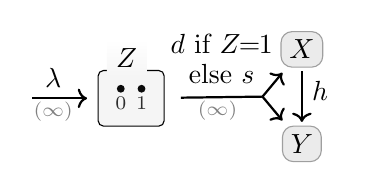
\begin{tikzpicture}[center base]
	% \node[dpad0] (Z) at (-0.2,0) {$Z$};
	\node[tpt={z0|$0$}] at (-0.5,0.1) {};
	\node[tpt={z1|$1$},right=0.15 of z0]{};
	\node[Dom={$Z$[label distance=-1.5ex, xshift=1.0em] (Z)
		around {\lab{z0}\lab{z1}}} ] {};

	% \node[dpad0,align=center] (XY) at (1.8,0) {$XY$}; %{$X$\\[-0.3ex]$Y$};
	\node[dpad0] (X) at (1.8, 0.6) {$X$};
	\node[dpad0] (Y) at (1.8, -0.6) {$Y$};
	\coordinate (xyz) at (1.3, 0);
	\draw[arr1, <-] (Z) to
		node[above, pos=0.6]{$\lambda$}
		% node[above, pos=0.6]{$\frac{1}{\lambda_0+\lambda_1}[\lambda_0, \lambda_1]$}
		node[below,inner sep=1pt, pos=0.6]{${\color{gray}\scriptstyle( \infty )}$}
		+(-1.3, 0);
	% \node at (-1,-0.6) {\small where $\lambda(Z) = \frac{\lambda_Z}{\lambda_0+\lambda_1}$};
	% \node at (0,-0.6) {\small where $\lambda(Z) \propto \lambda_Z$};
	\draw[arr1] (X) to node[right,pos=0.4]{$h$} (Y);
	\draw[arr,-,shorten >=0pt] (Z) to[bend left=0, shorten >=0pt]
		% node[fill=white, inner sep=0pt, pos=0.55]
		% node[inner sep=1pt, pos=0.55]
		node[above, inner sep=1pt, pos=0.55]
			% {$Z?d:s$}
		% {$\begin{bmatrix}d \text{ if } Z\\[-0.3ex] s \text{ else}\end{bmatrix}$}
		{$\begin{matrix}d \text{ if } Z\!\!=\!\!1\\[-0.3ex]
			% s \text{ else}\end{matrix}$}
			\text{else }s\end{matrix}$}
		% node[above, inner sep=2pt, pos=0.68]
		% 	{${\color{gray}\scriptscriptstyle(r)}$}
		node[below,inner sep=1pt]{${\color{gray}\scriptstyle( \infty )}$}
		(xyz);
	\draw[arr2, shorten <=0pt] (xyz) to (X);
	\draw[arr2, shorten <=0pt] (xyz) to (Y);
\end{tikzpicture}
% \text{where }
% \lambda(Z) =  \frac{1}{\lambda_0\!+\!\lambda_1}
% \begin{bmatrix}
% 	\lambda_0 \\\lambda_1
% \end{bmatrix}
\qquad
\dg M_2 :=
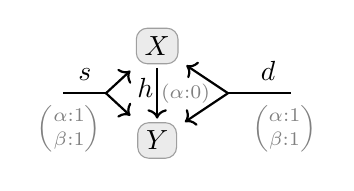
\begin{tikzpicture}[center base]
	\node[dpad0] (X) at (0, 0.6) {$X$};
	\node[dpad0] (Y) at (0, -0.6) {$Y$};
	\draw[arr1] (X) to node[left=0pt,pos=0.4, inner sep=1pt]{$h$}
			% node[below=0pt,inner sep=1pt,rotate=90]{${\color{gray}\scriptstyle(\!\alpha{:}0\!)}$}
			node[right=0pt,inner sep=1pt]{${\color{gray}\scriptstyle(\alpha{:}0)}$}
		(Y);

	\coordinate (d0) at (1.8, 0);
	\coordinate (s0) at (-1.3, 0);
	\node[above left=1pt and 0.5em of d0] {$d$};
	\node[below left=0pt and -1em of d0]{${\color{gray}\scriptstyle
		\renewcommand{\arraystretch}{.8}
		\begin{pmatrix} \scriptstyle\alpha: 1 \\[-0.2ex] \scriptstyle\beta:1 \end{pmatrix}}$};
	\node[above right=1pt and 0.5em of s0] {$s$};
	\node[below right=0pt and -1em of s0]{${\color{gray}\scriptstyle
		\renewcommand{\arraystretch}{.8}
		\begin{pmatrix}\scriptstyle
		\alpha: 1 \\[-0.2ex] \scriptstyle \beta: 1 \end{pmatrix}}$};

	\unmergearr{s0}XY
	\unmergearr{d0}XY
% 	\draw[arr,-,shorten >=0pt] (Z) to[bend left=0, shorten >=0pt]
% 		node[fill=white, inner sep=0pt, pos=0.55]
% 			% {$Z?d:s$}
% 			{$\begin{bmatrix}d\\[-0.3ex] s\end{bmatrix}$}
% 		% node[above, inner sep=2pt, pos=0.68]
% 		% 	{${\color{gray}\scriptscriptstyle(r)}$}
% 		(xyz);
% 	\draw[arr2, shorten <=0pt] (xyz) to (X);
% 	\draw[arr2, shorten <=0pt] (xyz) to (Y);
% ode[dpad0] (X) {};
\end{tikzpicture}
\qquad
% \dg M_2 :=
% \begin{tikzpicture}
% 	\node[dpad0] (X) {};
% \end{tikzpicture}
% \qquad
\dg M_3 :=
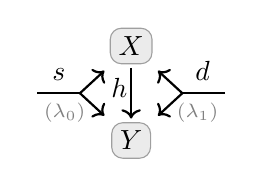
\begin{tikzpicture}[center base]
	\node[dpad0] (X) at (0, 0.6) {$X$};
	\node[dpad0] (Y) at (0, -0.6) {$Y$};
	\draw[arr1] (X) to node[left=0pt,pos=0.4, inner sep=1pt]{$h$} (Y);

	\coordinate (d0) at (1.3, 0);
	\coordinate (s0) at (-1.3, 0);
	\node[above left=1pt and 0.5em of d0] {$d$};
	\node[below left=0pt and 0.2em of d0]{${\color{gray}\scriptstyle( \lambda_1 )}$};
	\node[above right=1pt and 0.5em of s0] {$s$};
	\node[below right=0pt and 0.2em of s0]{${\color{gray}\scriptstyle( \lambda_0 )}$};

	\unmergearr{s0}XY
	\unmergearr{d0}XY
% 	\draw[arr,-,shorten >=0pt] (Z) to[bend left=0, shorten >=0pt]
% 		node[fill=white, inner sep=0pt, pos=0.55]
% 			% {$Z?d:s$}
% 			{$\begin{bmatrix}d\\[-0.3ex] s\end{bmatrix}$}
% 		% node[above, inner sep=2pt, pos=0.68]
% 		% 	{${\color{gray}\scriptscriptstyle(r)}$}
% 		(xyz);
% 	\draw[arr2, shorten <=0pt] (xyz) to (X);
% 	\draw[arr2, shorten <=0pt] (xyz) to (Y);
% ode[dpad0] (X) {};
\end{tikzpicture}
\qquad
\]
\vspace{-2ex}

% A second approach: use something like
% % $\mathcal L = \sum_{x\sim } h(y|x) \log \frac{h(y|x)}{d(y|x) q(y|x)}$
% $\smash{\Ex_{x\sim m} h(y|x) \log \frac{h(y|x)}{d(y|x) q(y|x)}}$.
Our practitioner now tries a different approach: draw data samples $(x,y) \sim d$ but discount $h$'s surprisal when the simulator finds the point unlikely, via loss $\mathcal L_2 := \Ex_{d} [s(\mkern-2muX\!,\!Y\mkern-2mu) \log \nf1{h(Y|X)}]$.
This is the cross entropy with respect to the (unnormalized) product density $ds$, which in many ways is appropriate.
However, by this metric, the optimal predictor $h^*(Y|x) \propto d(Y|x) s(Y|x)$ is uncalibrated.
If the data and simulator agree ($d \!=\! s$), then we would want $h(Y|x) \!=\! s(Y|x)$ for all $x$, but instead we get $h^*(Y|x) \propto s(Y|x)^2$.
So $h^*$ is overconfident.
What went wrong?
% $\mathcal L_2$ is not easily written as an inconsistency using $s,h,$ and $d$, but it can be written as the 1-inconsistency
% $\mathcal L_2$ cannot be written as an inconsistency unless we also take the quailtative score into account, in which case it equals $\aar{\dg M_2}_1$.
% $\aar{\dg M_2 \text{ with } \alpha_d,\alpha_s \!:=\!1;~\alpha_h\!:=\!0}_1$.
% $\aar{\dg M_2 \text{ with } \alpha_d,\alpha_s \!:=\!1;~\alpha_h\!:=\!0}_1$.
% Although $\balpha$ is not the focus of the present paper, these values are problematic: they indicate an overdetermination of $X \times Y$, and as a consequence $h^*$ is more deterministic than it should be.
The simplest PDG account of $\mathcal L_2$ is the 1-inconsistency $\aar{ \dg M_2 }_1$, but the values of $\balpha$ in $\dg M_2$ indicate an over-determination of $XY$ (it's determined in two ways),
  and so $h^*$ is more deterministic than it should be.
By contrast, $\aar{\dg M_3}$ does not have this issue: its optimal $h$ is proportional the $\lambda$-weighted geometric mean of $s$ and $d$.
% Both losses of the initial approach also arise from PDGs, and the lack of calibration in the second stems from strange modeling assumptions.
The discussion at the end of \S8 and Appendix C.1.2 gives another calibration example.
% We will add this example to the appendix as well.
% This example addresses Reviewer \#3's concern: thinking about what's going on is more than pedagogy; it is a valuable first step in the modeling workflow!
% For \revc{Reviewer \#4}: viewing losses through the same lens like this makes it possible to analyze and choose loss functions uniformly, as we say in the introduction.
% To address \revc{Reviewer #3}: this ; describing what's going on is a valuable safeguard first step in the modeling workflow.
To address \revc{Reviewers \#3 and \#4}: this unified view can suggest more appropriate loss functions and better approaches to a problem; clear thinking is not just about pedagogy.
% In our telling, this is backwards, since the losses of both approaches also come from PDGs, but less reasonable ones


% \textbf{With a PDG.}
% the Bhattacharya distance: a loss that is much smaller if the t. does not generate a training point ($\exists x. p(x) \ll q(x)$).
% % the Bhattacharya distance: a symmetric measure that punishes cases where the model does not generate a training point ($p \ll q$) less severely.
% % the Bhattacharya distance: a loss that punishes cases where the model does not generate a training point ($\exists x. p(x) \ll q(x)$) less severely.
%
% If the $\beta_s = \beta_q$, then the loss function that arises are
% If the $p,q$ have corresponding confidences $\beta_p$ and $\beta_q$, then the cpd $h(Y|X)$ that minimizes the inconsistency will be proportional to $p(Y|X)^{\beta_P} q(Y|X)^{\beta_q}$.
% So, it will be smaller if there's



% \textbf{Cases where PDGs and the Standard Diverge.}
% \textbf{Discrepency betwen PDG inconsistency and common losses.}
% % Reviewers \#4 and \#5 ask for an example where the PDG gives a non-standard loss that is in some sense better than what a practitioner might think to use.
% Reviewers \#4 and \#5 ask for a practical example in which it is common to use one function, but a different, (better) one arises from the appropriate PDG.
% % Before that, we'd like to first give the field some credit: in settings where a loss function is standard, it is usually for good reason.
% First, we'd like to give the field credit: in settings where a loss function is standard, it is usually for good reason.
%
%
%%% REVIEW: Fold back in?
% Our experience suggests that minimizing the inconsistency of the appropriate PDG is always desirable, but is sometimes impractical. It may not have a closed-form expression, or be expensive to compute (e.g., the marginal surprisal in Prop 4, if $|\V(Z)|$ is large).
% Yet, as in Section 6.1, PDGs can still clarify the extra modeling assumptions we make for tractability.
%% Yet, as in Section 6.1, PDGs can still describe the modeling assumptions we use to gain tractability.

% % Now for the examples: one non-standard, and one impractical.
% Now for the examples.
% Suppose we would like to train a predictor network $h(Y|X)$ a partially corrupted emperical distribution $d(X,Y)$, and an analytical model $q(X, Y)$.
% One first approach in applied ML might be to use the sum of the two cross entropies:
% % $- 2 \Ex_{x,y \sim {\nf12(d + q)}} \log h(y|x)$. This fits $h$ to the mixture $\frac12 (d + q)$,
% $- 2 \Ex_{m} \log h(Y|X)$, where $m := \nf12(d + q)$.
% This loss fits $h$ to $m$, effectively
% treating $d$ and $q$ as disjoint; the redundancy is not used to correct errors.


\textbf{Motivating VAEs.}
\revc{Reviewer \#3} points out that a VAE is already associated with a graphical model.
% While this is true, that graphical model is only a simple Bayesian Network made up of the prior and decoder; and encodes neither the encoder nor the loss function---it is associated with the VAE for good reason, but falls short of capturing it.  Our observation: simply include the encoder in addition (as is only possible in a PDG), and one also captures the loss function for free.
While this is true, that graphical model only partially describes the VAE, as it consists of the prior and decoder, but not the encoder.
% Our observation: simply include the encoder as well, as is only possible in a PDG, since the encoder and prior might be inconsistent with each other), to also obtains the loss function for free.
Only with a PDG can we model both the prior and encoder, as the two might be inconsistent.
Moreover, we get the loss function for free by doing so, as the resulting inconsistency.
%
%TODO: do I want space here?
%
\revc{Reviewer \#3} also pushes back on our claim that the ELBO is difficult to motivate,
% with reference to
citing
the fact that the ELBO is a tractable lower bound on the log likelihood (a simple derivation that we review in Section 6.1).  This is indeed the standard motivation,
but it is arguably incomplete---%
% but we find it unsatisfying---%
% the constant
% % $-\infty$
% \texttt{FLOAT\_MIN}
a constant encoding the smallest representable number on a computer
% satisfies these criteria,
is a tractable lower bound,
but still a poor loss function.
Of possibly many lower bounds, why use this one? What does the ELBO represent?
% Does it have units?
Why is it negative?
Why use the logarithm instead of another concave function?
% There are good answers to these questions, but not, in our view, simple ones.
Such questions are all easy to answer with PDG semantics. There are other answers to these questions, but not, in our view, simple ones.


\textbf{What Now?} \revc{Reviewers \#5 and \#6} wonder where to go from here. Among other things, we are working out solid grounding of $\balpha$ in causality,  tractable inference algorithms for PDGs, and a view of probabilistic databases as PDGs.


% \textbf{A PDG Modeling Workflow.}
% Reviewer \#3 asks whether there's a contribution here beyond pedagogy that could aid learning or inference.
% Reviewer \#4 wants more discussion on the advantages of seeing losses through the same lens,
% while Reviewer \#6 wonders where to go from here.
% %
% We think it possible that PDGs will replace the entire modeling workflow.
% Beyond what we've shown here, PDGs can already describe network architectures, datasets, straight-line code.
% % We suspect we will also be able to fold in databases
% % And, unlike other approaches, one can design them from the middle outwards, without always needing to have a consistent data-generating process.
% Unlike other approaches, they can be easily recombined, built from the middle outwards, without a consistent data-generating process.
% What's missing, of course, are automated inference procedures, and tooling.
% On its own, this paper may be only good for pedagaogy and for defending a choice of loss function---but stay tuned.

% \usebibliography
\end{document}
